%-*- mode: latex; fill-column: 70 -*-
% ex: set sts=4 ts=4 sw=4 et tw=70:
%&pdflatex

\documentclass[letterpaper,landscape]{report}
\usepackage[landscape,margin=0.5cm]{geometry}
\usepackage{color}
\usepackage{flowfram}
\usepackage[colorlinks]{hyperref}

\usepackage{multicol}
\setlength{\columnseprule}{1pt} % for visible divider
\setlength{\columnsep}{1cm}

\usepackage{graphicx}
\graphicspath{
 {../}
}

\usepackage{enumitem}           % useful for control of listings

\pagestyle{empty}
\begin{document}

%%
%% DEBIAN
%%
\begin{multicols}{3}    % 3 columns

\begin{center}
\noindent
\includegraphics[width=0.5\columnwidth]{openlogo}

\url{http://www.debian.org}
\section*{Debian GNU/Linux}
\subsection*{The Universal Operating System}
\end{center}

\section*{Reasons to choose Debian}
\paragraph{It is maintained by its users}
If something needs to be fixed or improved, we just do it.

\paragraph{Unparalleled support}

Mail sent to the mailing lists often gets answers within 15 minutes (or less),
for free, and by the people who developed it. Compare that to typical phone
support: hours spent on the phone, for money, only to get someone who doesn't
know the system well enough to even understand your question.

\paragraph{You wouldn't be alone in your choice}

A wide range of organizations and individuals use Debian. See our Who's Using
Debian? page for a description of some high-profile sites which use Debian, and
have chosen to submit a short description of how they use Debian and why.

\paragraph{The best packaging system in the world.}

Tired of old files from software three versions old cluttering your system? Or
installing a piece of software only to find it causes your system to crash
because of software conflicts? Dpkg, Debian's endured packaging system, takes
care of these issues for you.

\paragraph{Easy installation}

If you have heard that GNU/Linux is difficult to install, then you haven't
tried Debian lately. We are constantly improving the installation process. You
can do the installation directly from CD, DOS, floppies or even over the
network.

\paragraph{Incredible amounts of software}

Debian comes with over 25000 different pieces of software. Every bit of it is
free. If you have proprietary software that runs under GNU/Linux, you can still
use it - in fact, there may even be an installer in Debian that will
automatically install and set up everything for you.

\paragraph{Packages well integrated}

Debian surpasses all other distributions in how well its packages are
integrated. Since all software is packaged by a coherent group, not only can
all packages be found at a single site, but you can be assured that we have
already worked out all issues regarding complicated dependencies. While we feel
that the deb format has some advantages over the rpm format, it is the
integration between the packages that makes a Debian system more robust.

\paragraph{Source code}

If you are a software developer, you will appreciate the fact that there are
hundreds of development tools and languages, plus millions of lines of source
code in the base system. All of the software in the main distribution meets the
criteria of the Debian Free Software Guidelines (DFSG). This means that you can
freely use this code to study from, or to incorporate into new free software
projects. There are also plenty of tools and code suitable for use in
proprietary projects.

\paragraph{Easy upgrades}

Due to our packaging system, upgrading to a new version of Debian is a snap.
Just run apt-get update ; apt-get dist-upgrade (or aptitude update; aptitude
dist-upgrade in newer releases) and you can upgrade from a CD in a matter of
minutes or point apt at one of the over 300 Debian mirrors and upgrade over the
net.

\rotatebox{90}{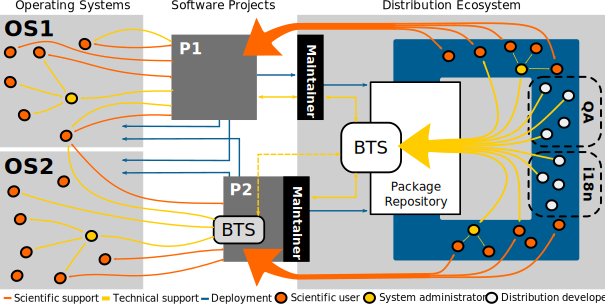
\includegraphics[height=.9\columnwidth]{distro-dev}}
\rotatebox{90}{Description}

\paragraph{Multiple architectures and kernels}

Currently Debian supports an impressive number of CPU architectures: alpha,
amd64, armel, hppa, i386, ia64, mips, mipsel, powerpc, s390, and sparc. It also
runs on GNU Hurd and FreeBSD kernels besides Linux, and with the debootstrap
utility you will be hard-pressed to find a device that can't run Debian.

\paragraph{Bug tracking system}

Debian's bug tracking system is publicly available. We don't try to hide the
fact that software doesn't always work the way users want. Users are encouraged
to submit bug reports and are notified when and why the bug was closed. This
system allows Debian to respond to problems quickly and honestly.



\section*{Acknowledgements}

\end{multicols}


\pagebreak
%%
%% NeuroDEBIAN
%%
\begin{multicols}{3}    % 3 columns

\begin{center}
\noindent
\vspace{-3em}
\includegraphics[width=\columnwidth]{logo_tuned/label}

\url{http://neuro.debian.net}
\section*{NeuroDebian Project}
\subsection*{The Universal Research Environment}


\end{center}

\section*{What is NeuroDebian}

\section*{What is in NeuroDebian}

Icons for FSL, Caret, AFNI, etc


%\columnbreak

\section*{How to get NeuroDebian}

\begin{itemize}
\item Debian/Ubuntu -- Repository
\item Others -- Virtual Appliance
\end{itemize}

\section*{Developers oriented information}

buga dugabuga dugabuga dugabuga dugabuga dugabuga dugabuga dugabuga dugabuga dugabuga dugabuga dugabuga dugabuga dugabuga dugabuga dugabuga dugabuga dugabuga dugabuga dugabuga dugabuga duga
sdflkj
slkdjf

%\columnbreak

\section*{Who is using NeuroDebian}

\noindent
%\includegraphics[width=\columnwidth]{usage_worldmap}

buga dugabuga dugabuga dugabuga dugabuga dugabuga dugabuga dugabuga dugabuga dugabuga dugabuga dugabuga dugabuga dugabuga dugabuga dugabuga dugabuga dugabuga dugabuga dugabuga dugabuga duga


\section*{Future\ldots}

\begin{description}[leftmargin=1em]

\item[Wider coverage]:\\
  BioSig, NEURON, FreeSurfer, etc.

\item[Assured interoperability]:\\
  Intergration- and regression- testing

\item[Snapshotting]

\item[Data as 1st class citizen]

\item[Universal Availability]:\\
  \begin{itemize}
  \item New versions of Virtual Appliance
  \item Cloud computing images
  \end{itemize}

\end{description}


\section*{Endorsements}

some quotes from letters of support


\section*{Acknowledgements}

We are grateful to all Debian developers and contributors for the
development of Debian OS, and to Prof. Jim Haxby (PBS Department,
Dartmouth College) for his continued support and endless supply of
Italian espresso.

%\columnbreak
\end{multicols}



\end{document}


%%% Local Variables:
%%% mode: latex
%%% TeX-master: t
%%% TeX-PDF-mode: t
%%% whizzy-viewers: (("-pdf" "okular") ("-dvi" "xdvi") ("-ps" "gv"))
%%% End:
